\documentclass[tikz]{standalone}
\usetikzlibrary{spy,shapes,shadows,calc,pgfplots.groupplots}
\usepackage{amsmath}
\usepackage{physics} 
\usepackage{pgfplots}
\pgfplotsset{compat=1.3}
\usepackage{amsmath}
\DeclareFontFamily{OT1}{pzc}{}
\DeclareFontShape{OT1}{pzc}{m}{it}{<-> s * [1.10] pzcmi7t}{}
\DeclareMathAlphabet{\mathpzc}{OT1}{pzc}{m}{it}
\newcommand{\ddtn}{\operatorname{dtn}}

\pgfplotsset{
  legend style = {font=\small}
}

\begin{document}
\begin{tikzpicture}[scale = 1.0]

%\begin{axis}[
\begin{groupplot}[
    group style={
        %group name=dtn,
        group size=3 by 1,
        %xticklabels at=edge bottom,
        horizontal sep=5pt,
        vertical sep=40pt,
   },
   %name = dtnplot,
   height = 6cm,
   width = 7.0cm,
   every axis plot/.append style={thick},
   axis y line*=left,
   legend pos = south east,
   %xmin = 0,
   %xmax = 11000,
   %ymin = -20,
   %ymax = 20,
   %restrict y to domain=-1e2:1e2,
   %label style={at={(axis description cs:0.5,-0.08)},anchor=north},
   %every x tick scale label/.style={at={(xticklabel cs:0.925)},anchor=south west},
   x label style={at={(axis description cs:0.75,0.085)},anchor=east},
   %xlabel= { $\lambda$},
    ymin = 3e-5,
    ymax = 3e-1,
   ]
    \nextgroupplot[ 
    ymode=log,
    xmode=log,
    %xmin=0,xmax=1.6e4,
    %xtick={25, 125, 250, 500, 800, 1000},
    %axis x line*=middle,
    %axis y line=middle, 
    %ymin = 1e-5,
    %ymax = 4e0,
    %width=9cm,
    %restrict y to domain=-4e2:4e2,
    %xtick={0,2e3,4e3,6e3,8e3,10e3,12e3,14e3},
    xlabel= {ndof},
    %legend pos = south west,
    legend pos = south west,
    %x label style={at={(axis description cs:0.575,-0.15)},anchor=east},
    title = { $ (\mu_1,\mu_2) = (2,20) $ }, 
    %y tick label style={xshift={3em}}
	]

    \addplot[red,very thick,mark=*,forget plot] 
   	table[x=ndof,y=rel-L2-err-B] {../data/ball-4-norm-squares-iprelL2error-pq1-mus(2,20)-ks(0,0).dat}; 
    \addplot[blue,very thick,mark=triangle,forget plot]  
	table[x=ndof,y=rel-L2-err-B] {../data/ball-4-norm-squares-iprelL2error-pq2-mus(2,20)-ks(0,0).dat}; 
    \addplot[green!70!black,very thick,mark=x,forget plot]  
   	table[x=ndof,y=rel-L2-err-B] {../data/ball-4-norm-squares-iprelL2error-pq3-mus(2,20)-ks(0,0).dat}; 
    \addplot[gray,dotted,thick,forget plot] 
   	table[mark=none,x=ndof,y expr ={1.5e0*\thisrowno{1}}] {../data/ball-4-norm-squares-iprelL2error-pq1-mus(2,20)-ks(0,0).dat}; 
    \addplot[gray,dashed,thick,forget plot] 
   	table[mark=none,x=ndof,y expr ={3e1*\thisrowno{1}*\thisrowno{1}}] {../data/ball-4-norm-squares-iprelL2error-pq3-mus(2,20)-ks(0,0).dat}; 
    
    \node (mypic) at (axis cs:2e3,4.5e-4) {
\includegraphics[scale = .095]{ball-4-norm-squares-p2q2-lvl4-mu-2-20-k-0-0.png}};
    \node[draw,circle,ultra thick,lightgray] (W1) at (axis cs:3.2e5,7.3e-4) {};
     \node[] (W2) at (axis cs:1.25e4,4e-4) {};
     \draw[lightgray,ultra thick,->] (W1.west) -- (W2.east);    
    %\legend{ ,$p=2$,$p=3$, $\mathcal{O}(h)$, $\mathcal{O}(h^2)$  } 	    
     
    \nextgroupplot[ 
    ymode=log,
    xmode=log,
    %xmin=0,xmax=1.6e4,
    %xtick={25, 125, 250, 500, 800, 1000},
    %axis x line*=middle,
    %axis y line=middle, 
    ymajorticks=false, 
    %ymin = 1e-5,
    %ymax = 4e0,
    %width=9cm,
    %restrict y to domain=-4e2:4e2,
    %xtick={0,2e3,4e3,6e3,8e3,10e3,12e3,14e3},
    %xlabel= {ndof},
    %legend pos = south west,
    legend pos = north east,
    %x label style={at={(axis description cs:0.575,-0.15)},anchor=east},
    title = {  $ (\mu_1,\mu_2) = (2,2) $  },
	]
    \node (mypicc) at (axis cs:2e3,4.5e-4) {
\includegraphics[scale = .095]{ball-4-norm-squares-p2q2-lvl4-mu-2-2-k-0-0.png}};
    \node[draw,circle,ultra thick,lightgray] (Z1) at (axis cs:3.2e5,3.9e-4) {};
     \node[] (Z2) at (axis cs:1.25e4,4e-4) {};
     \draw[lightgray,ultra thick,->] (Z1.west) -- (Z2.east);    
    
     \addplot[red,very thick,mark=*, forget plot] 
   	table[x=ndof,y=rel-L2-err-B] {../data/ball-4-norm-squares-iprelL2error-pq1-mus(2,2)-ks(0,0).dat}; 
    \addplot[blue,very thick,mark=triangle, forget plot]  
	table[x=ndof,y=rel-L2-err-B] {../data/ball-4-norm-squares-iprelL2error-pq2-mus(2,2)-ks(0,0).dat}; 
    \addplot[green!70!black,very thick,mark=x,forget plot]  
   	table[x=ndof,y=rel-L2-err-B] {../data/ball-4-norm-squares-iprelL2error-pq3-mus(2,2)-ks(0,0).dat}; 
    \addplot[gray,dotted,thick, forget plot] 
   	table[mark=none,x=ndof,y expr ={1.5e0*\thisrowno{1}}] {../data/ball-4-norm-squares-iprelL2error-pq1-mus(2,20)-ks(0,0).dat}; 
    \addplot[gray,dashed,thick,forget plot] 
   	table[mark=none,x=ndof,y expr ={3e1*\thisrowno{1}*\thisrowno{1}}] {../data/ball-4-norm-squares-iprelL2error-pq3-mus(2,20)-ks(0,0).dat}; 
    


    \nextgroupplot[ 
    ymode=log,
    xmode=log,
    %xmin=0,xmax=1.6e4,
    %xtick={25, 125, 250, 500, 800, 1000},
    %axis x line*=middle,
    %axis y line=middle, 
    ymajorticks=false, 
    %ymin = 1e-5,
    %ymax = 4e0,
    %width=9cm,
    %restrict y to domain=-4e2:4e2,
    %xtick={0,2e3,4e3,6e3,8e3,10e3,12e3,14e3},
    %xlabel= {ndof},
    %legend pos = south west,
    legend pos = north east,
    %x label style={at={(axis description cs:0.575,-0.15)},anchor=east},
    title = {  $ (\mu_1,\mu_2) = (20,2) $  },
    legend style = { column sep = 10pt, legend columns = 5, legend to name = grouplegend,},
	]

     \node (mypiccc) at (axis cs:2e3,4.5e-4) {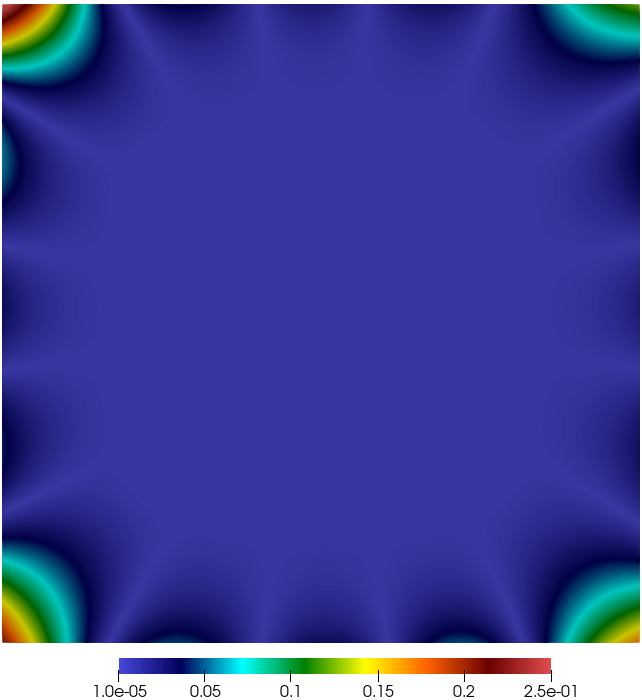
\includegraphics[scale = .095]{ball-4-norm-squares-p2q2-lvl4-mu-20-2-k-0-0.png}};
    \node[draw,circle,ultra thick,lightgray] (K1) at (axis cs:3.2e5,3e-4) {};
     \node[] (K2) at (axis cs:1.25e4,1e-4) {};
     \draw[lightgray,ultra thick,->] (K1.west) -- (K2.east);    
    
    \addplot[red,very thick,mark=*] 
   	table[x=ndof,y=rel-L2-err-B] {../data/ball-4-norm-squares-iprelL2error-pq1-mus(20,2)-ks(0,0).dat}; \addlegendentry{$ p = 1 $ }%
    \addplot[blue,very thick,mark=triangle]  
	table[x=ndof,y=rel-L2-err-B] {../data/ball-4-norm-squares-iprelL2error-pq2-mus(20,2)-ks(0,0).dat}; \addlegendentry{$ p = 2 $ }%
    \addplot[green!70!black,very thick,mark=x]  
   	table[x=ndof,y=rel-L2-err-B] {../data/ball-4-norm-squares-iprelL2error-pq3-mus(20,2)-ks(0,0).dat}; \addlegendentry{$ p = 3 $ }%
    \addplot[gray,dotted,thick] 
   	table[mark=none,x=ndof,y expr ={1.5e0*\thisrowno{1}}] {../data/ball-4-norm-squares-iprelL2error-pq1-mus(2,20)-ks(0,0).dat}; \addlegendentry{ $\mathcal{O}(h)$ }%
    \addplot[gray,dashed,thick] 
   	table[mark=none,x=ndof,y expr ={3e1*\thisrowno{1}*\thisrowno{1}}] {../data/ball-4-norm-squares-iprelL2error-pq3-mus(2,20)-ks(0,0).dat}; \addlegendentry{ $\mathcal{O}(h)$ }%
    %\node (geom) at (axis cs:1.5e3,3e-4) {\includegraphics[scale =.075]{meshes/squares-nrefs0-omega-B.pdf}};
    \end{groupplot}
    \node at ($(group c2r1) + (-0.0cm,-3.1cm)$) {\ref{grouplegend}};

\end{tikzpicture}
\end{document}












